%%%%%%%%%%%%%%%%%%%%%%%%%%%%%%%%%%%%%%%%%%%%%%%%%%%%%%%%%%%%%%%%%%%%%
%%%
%%% Set these variables appropriately
%%%
\newcommand{\AUTHORS}{pandas}
\newcommand{\TITLE}{Proxy Rotation with Bitcoin Micropayments}
\newcommand{\KEYWORDS}{}
\newcommand{\CONFERENCE}{}
\newcommand{\PAGENUMBERS}{yes}       % "yes" or "no"
\newcommand{\TOAPPEAR}{no}
%%%
%%%
%%%%%%%%%%%%%%%%%%%%%%%%%%%%%%%%%%%%%%%%%%%%%%%%%%%%%%%%%%%%%%%%%%%%%

%%%% Setup the document/page
\documentclass[pdftex,twoside,twocolumn,11pt,letterpaper]{article}
\usepackage{ifthen}

\ifthenelse{\equal{\PAGENUMBERS}{yes}}{%
\usepackage[nohead,
            left=1in,right=1in,top=1in,
            footskip=0.5in,bottom=0.75in     % Room for page numbers
            ]{geometry}
}{%
\usepackage[noheadfoot,columnsep=0.2in,
            margin=1in,centering,truedimen]{geometry}
}

\usepackage{fancyhdr}
\usepackage[numbers,sort]{natbib}
\usepackage{xspace}
\usepackage{booktabs}
\usepackage{subfigure}
\usepackage[T1]{fontenc}
\usepackage{textcomp}
\usepackage{mathptmx}   % Times + Times-like math symbols
\usepackage{courier}
\usepackage[scaled=0.92]{helvet}

\usepackage{color}
\usepackage[pdftex]{graphicx}
\ifthenelse{\isundefined{\wantBW}}{%
  \usepackage[colorlinks]{hyperref}%        % for online version
}{%
  \usepackage[pdfborder={0 0 0}]{hyperref}% % for paper (B&W) version
}
\newcommand{\URL}[1]{\url{#1}}

%%%%% Setup for PDF
\hypersetup{%
pdfauthor = {\AUTHORS},
pdftitle = {\TITLE},
pdfsubject = {\CONFERENCE},
pdfkeywords = {\KEYWORDS},
bookmarksopen = {true}
}

%\setlength{\parindent}{0pt}
%\setlength{\parskip}{0pt}
\renewcommand{\headrulewidth}{0pt}
\newcommand{\Paragraph}[1]{\vspace{-2ex}\paragraph{#1.}}
\setlength{\topmargin}{-.15in}

\ifthenelse{\equal{\PAGENUMBERS}{yes}}{%
  \pagestyle{plain}
}{%
  \pagestyle{empty}
}

\makeatletter\long\def\@makecaption#1#2{
   \vskip 10pt
   \setbox\@tempboxa\hbox{\textsf{#1: #2}}
   \ifdim \wd\@tempboxa >\hsize % IF longer than one line:
       \textsf{#1: #2}\par      % THEN set as ordinary paragraph.
     \else                      % ELSE  center.
       \hbox to\hsize{\hfil\box\@tempboxa\hfil}
   \fi}
\makeatother

\clubpenalty=10000  % Don't allow orphans
\widowpenalty=10000 % Don't allow widows

\title{\textbf{\TITLE}}
\author{\AUTHORS}
\date{}

% Compact itemize and enumerate.  Note that they use the same counters and
% symbols as the usual itemize and enumerate environments.
\def\compactify{\itemsep=0pt \topsep=0pt \partopsep=0pt \parsep=0pt}
\let\latexusecounter=\usecounter
\newenvironment{CompactItemize}
  {\def\usecounter{\compactify\latexusecounter}
   \begin{itemize}}
  {\end{itemize}\let\usecounter=\latexusecounter}
\newenvironment{CompactEnumerate}
  {\def\usecounter{\compactify\latexusecounter}
   \begin{enumerate}}
  {\end{enumerate}\let\usecounter=\latexusecounter}

\newcommand{\comment}[1]{\textcolor{red}{#1}}
\newcommand{\ignore}[1]{}

\newcommand{\xc}[1]{\mbox{\textit{#1}}}
\newcommand{\la}{\leftarrow}
\newcommand{\ra}{\rightarrow}
\newcommand{\somespace}{\hspace{0.1cm}}

\def\discretionaryslash{\discretionary{/}{}{/}}
\def\discretionarydot{\discretionary{.}{}{.}}
\def\discretionarycolon{\discretionary{:}{}{:}}
{\catcode`\/\active
\catcode`\.\active
\catcode`\:\active
\gdef\URLprepare{\catcode`\/\active\let/\discretionaryslash
                 \catcode`\.\active\let.\discretionarydot
                 \catcode`\:\active\let:\discretionarycolon
        \def~{\char`\~}}}%
\def\URL{\bgroup\URLprepare\realURL}%
\def\realURL#1{\tt #1\egroup}%

\newcommand{\eg}{{\em e.g.}, }
\newcommand{\ie}{{\em i.e.}, }
\newcommand{\etal}{{\em et al.\ }}

\def\check{\stackrel{{\scriptscriptstyle ?}}{=}}

\begin{document}
\maketitle

% -*-LaTeX-*-
% $Id: abstract.tex 70 2007-01-30 21:59:16Z nicolosi $

\begin{abstract}
ABSTRACT HERE
\end{abstract}

   
\section{Introduction}
\label{sec:intro}

Proxies are a powerful to for tasks such as browsing privately and evading censorship. The number of available proxy services on the internet is limited, in part due to lack of incentive for servers to operate. This means it is difficult for users to take advantage of more demanding techniques which require a number of proxies rather than a single one. We offer a solution to this problem by incentivizing proxy servers to join the network through use of Bitcoin micropayments. 

\subsection{Proxies}

One technology associated with proxies is proxy rotation, where a user rotates over a number of different proxies rather than just using one. This allows a user to appear to be many different machines rather than a single computer, hiding traffic from the user's session. This is currently used by web crawlers in order to avoid being blocked by a website by appearing to come from many different IP addresses. With some extension this technique can be applied to general proxy usage. There already exist some proxy services which use a similar model of owning many proxies and rotating a user's traffic through them, but this has the disadvantage of still being centralized on the business entity controlling the proxies.

\subsection{Background on Bitcoin}

Bitcoin\cite{nakamoto2008bitcoin} is a P2P digital currency which has exploded in popularity in the past few years. One of the appeals of Bitcoin is that online transactions do not require third party payment processors. Instead transactions can be included in a global history, called the block chain, in minutes. Additionally, transactions are not strongly tied to a person's identity, as is the case of credit card transactions, but rather tied to a pseudonymous address. Most transactions simply transfer Bitcoins from one address to another, but more complicated types of contracts can be built out of these transactions. We explore how one type of contract, micropayment channels, can be used to facilitate a proxy network. A micropayment channel allows an individual to make small incremental payments to another individual without actually posting a transaction to the block chain. For this case, we have applied micropayment channels so a client will increment their payment to a server when the server provides a service to them. When the channel is closed, a single transaction is posted, resolving many small transactions without publishing each of them on the block chain. Micropayments enable pay as you go type services where payment is immediate and does not suffer from transaction fees.

Although Bitcoin micropayments were first added to the Bitcoin Wiki by core Bitcoin developer Mike Hearn in December 2011,  actual deployment of micropayment based services has been very slow. No observable development happened until June 27, 2013 when BitcoinJ, a prominent java library for Bitcoin, added support for micropayments. Since then some services have been built using micropayments, but these are all specialized services, and these are still very few in number.

\section{Design}
\label{sec:design}

\subsection{Mechanics of Micropayment Channels}

Micropayments go through an initialization phase in which the client creates (but does not broadcast) an escrow transaction with the maximum amount of spendable money in the channel, requiring both the client's and the server's signatures to unlock. Next, the client creates a refund a refund transaction which recovers all of the money in escrow and is time locked (it will only be valid after a certain number of blocks have been mined, which can be approximated with a time as each block takes an average of 10 minutes to mine). The server then signs the refund transaction. 

After receiving the signed refund transaction, the client can then safely broadcast the previously created escrow transaction on the Bitcoin network. This marks the beginning of the payment phase. The client will sign transactions paying incrementally more money from the escrow to the server, and returning less money to themselves. These transactions are all double-spends off of the escrow transaction so only one can be validly placed on the block chain.

At some point the business between the client and the server comes to an end, bringing about the start of the final, resolution, phase. The most typical ending of business involves the client telling the server that they are done. At this point, the server will sign the payment provided by the client which gives the server the largest amount of money and broadcast it to the Bitcoin network.

\subsection{Advantages of the micropayment Structure}

There are a few major advantages to using Bitcoin micropayments. First, the micropayments are low risk for both the client and the server. In the initialization phase, the client does not broadcast the escrow transaction until they have a signed refund transaction from the server. This presents the client with no risk because if the server doesn’t behave or fails, the client can wait for the lock time to expire recover all of their coins from escrow. Also, the server has no reason to not sign the refund transaction because it only spends funds that already belong to the client.

During the payment phase, neither the server nor the client are at much risk. If the server stops providing service, the client will stop sending the new transactions with increased payment. Similarly, if the client stops sending new transactions, the server can stop providing its service. At the worst, the server or the client can only be cheated out of either one unit of service (eg megabyte of bandwidth), or one unit of payment.

The resolution phase can start in a few different ways other than the one discussed in the previous subsection. If the server doesn’t hear an updated transaction from the client for a long period of time, it will assume the client is done and close the connection, moving to the resolution phase. Additionally, the server will move to the resolution phase if the current time becomes too close to the unlock time for the refund transaction. If the server fails, the resolution phase consists of the client waiting to be able to post the refund transaction. This protects the client from an unresponsive server. An additional benefit of the micropayment structure is that it can be used to pay for arbitrarily small amounts of service (for proxy rotation, the units of service still need to be large enough that the overhead of the Bitcoin transactions doesn't dominate the data flow). This is useful as a single unit of service/payment is the risk being taken on by the server/client.

\subsection{Drawbacks of Micropayments bitches}

There are a few drawbacks associated with the micropayment structure. First, 
the client and server must deal with the confirmation time of transactions in Bitcoin. When the client makes the original escrow transaction, the server must wait for the transaction to be confirmed before it starts serving the client. If the server does not wait for the transaction to be confirmed, the client could attempt to double spend the money in the escrow, taking the money out of the payment channel. If this were to happen, the server would not be paid for the service it had already provided (making the risk larger than one service increment). This means that the escrow needs to be set up in advance of the client using the proxy. 

Another small drawback of the micropayment structure is that even though a client will recoup their funds from escrow eventually (from a dead server), they must wait for the refund transaction to become available. Currently, the waiting period is set to 24 hours, which means that a client’s money would be unavailable for this time. If a client puts a lot of money in escrow with several derelict servers, they can cause a large amount of their funds to become temporarily frozen.


\subsection{Financial Design and Motivation}

Currently the available proxy market is made up of free proxies which are slow, with bad availability, and paid proxies which use per-month credit card payments. The lack of quality in free proxies can be a problem. It has been shown that the Tor relays have a lopsided distribution with more than expected residing in less stable IP prefixes \comment{(reference: Jen's paper)}. Using credit cards to pay for proxies also has its problems and reduces the anonymity of a user, as each proxy a user shares their identifying information with could be infiltrated by an attacker or seized by an adversary with state powers. Using month to month proxies also limits the pool size of proxies due to the practical financial limitations on how many proxies a single person could afford to be subscribed to in a single month. 

We would like to employ a third economic strategy, involving Bitcoin, to bring many parties to the market, on both the client and proxy side. Using Bitcoin for payment to proxies provides significant benefits over free proxies or pay by month proxies. As opposed to free proxies, using Bitcoin micropayments could make proxies much more available. Once servers are collecting a small fee, it is in their interest to maintain a certain quality of service. Specifically, the Bitcoin fees could be configured in such a way as to charge per byte. Thus, a server would make more money if it was quick (an incentive to be fast), and would only be paid if it was functioning (an incentive to be available). When compared to credit card subscriptions, the Bitcoin payment method also has advantages. Bitcoin is a pseudonymous payment system, which allows payment to a proxy without revealing the identity of the client. It also makes the relationship between a client and a server short. This is particularly desirable for the client if the client is trying to evade oppressive censorship and the proxy constantly runs the risk of being shut down at some point before the payment period ends (in which case the client would lose out on a service they have already paid for).

\subsection{Discovery}

The proxy servers will be running, each listening on their respective port and IP addresses. Clients need a means of locating these proxy servers. We developed two methods for a client to discover proxies.
The first method involves using a BitTorrent tracker. A BitTorrent tracker is typically used by BitTorrent clients in order to find peers to download files from. A torrent client will connect to a tracker and send an announce request. The request will include a hash of the files the client is seeking. The tracker will then send an announce response to the client with a list of peers who also have that file, based on the info hash given. In our BitTorrent discovery implementation, we created a random “magic number” hash that all clients and proxies would announce to a bittorrent tracker. This way the tracker's announce responses will always include the IP addresses and ports of proxies.

The second method we employed is the Bitcoin block chain itself. The Bitcoin block chain stores a record of all transactions in the Bitcoin system. Typical transactions describe where the Bitcoins are coming from and where they are going, but some transaction types can be filled with 40 bytes of data. Forty bytes of data is sufficient to store an IP address and port number, but it would be impractical to interpret every 40 bytes of data on the block chain as an IP address and port (as the 40 bytes could be unrelated data). In order to detect which bytes can be interpreted as IP addresses and ports, proxy hosts will prefix the bytes of the IP address and port they are advertising with a magic number of sufficient length such that it is unlikely that the magic number appears in the normal operation of Bitcoin. The cost for a proxy to announce via Bitcoin is the transaction fee, plus a miniscule amount of Bitcoin, as the Bitcoin network doesn't accept transfers of zero Bitcoin.

The advantages of using a tracker based system is that the protocol is much simpler and doesn't require spending Bitcoins to advertise. An announcement to a BitTorrent tracker takes time on the order of seconds, whereas it takes an average of 10 minutes for a Bitcoin block to be mined. This causes a larger delay for proxies who are trying to bootstrap themselves. Thus, using trackers require less time and money for a proxy to get bootstrap. Another advantage of trackers is that there can be many trackers, as any existing tracker can now become a means of proxy discovery, or people could even run their own trackers on a smaller scale. Censors would have a harder time finding and eliminating all proxies or trackers.

On the other hand, just as it may be difficult for censors to find trackers, it may be hard for individuals to find trackers. The Bitcoin block chain provides an eventually consistent but decentralized means of storing and viewing information, meaning information on the block chain is hard to block but easy to find. To block the block chain discovery it would likely be necessary to block the Bitcoin protocol, which could be circumvented with format transforming encryption. Another option would be for censors to parse the announce messages on the block chain themselves, and censor all the addresses they find, but this could be abused by advertising arbitrary services, which would essentially force the censor to use a whitelist
.

\begin{figure*}
  \centering
  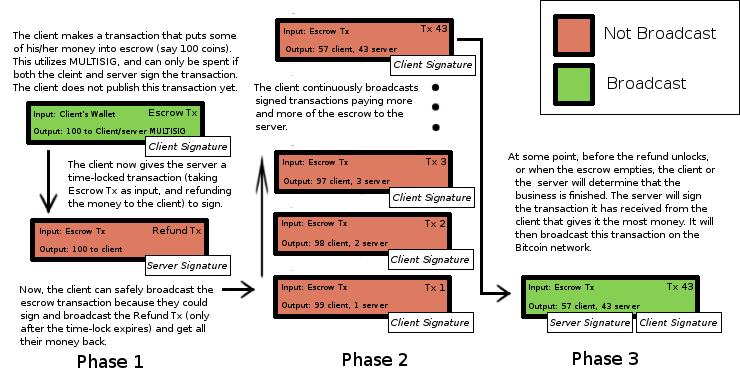
\includegraphics[width=0.95\textwidth]{microtransactions.png}
  \caption{Diagram of micropayment protocol}
\end{figure*}

\section{Implementation}
\label{sec:eval}

In this section we describe the design and creation of a basic prototype of our proxy system. Our goal was to implement two different programs: a local proxy that clients of the proxy network make use of and a server proxy that clients connect to. Both proxies act as SOCKS servers as well as Bitcoin wallets. When the client turns on, it discovers a set of active proxy servers, opens payment channels to them, and begins rotating its traffic over the active servers. It gradually pays for traffic as it requests pages. A user makes use of the client by directing their machine to tunnel traffic through the SOCKS server running locally.

\subsection{Dependency Stack}
We locally deployed a large stack of software in order to run and test our system without outside dependencies. For the BitTorrent based discovery system we ran a UDP tracker, UDPT. In order to test local Bitcoin network, we used the Bitcoind utility in regression test mode, which allows you to create and mine on a private block chain locally on your own computer. This allowed us to run all our tests without spending real Bitcoins or waiting for block mining and propagation delays. 

On top of this base layer of infrastructure we assembled our system on top of two distinct projects, Java Socks Proxy Server, a SOCKS 4 and SOCKS 5 proxy server written in Java, and BitcoinJ, a Java implementation of the Bitcoin protocol.

\subsection{Proxy Development}
We began by implementing the pure proxy section of the system without the payment system included. The main section of the program was exactly the same for the client and the server. The only difference being that the server forwards traffic directly to its destination whereas the client chooses a proxy server to tunnel requests through. This was achieved by using the Java class \texttt{ProxySelector}. This allowed us to dynamically decide which proxy to use every time a connection is made to a server. The class nicely encapsulated our code, allowing us to incorporate our client system into any sort of local server or application.

\subsection{Bitcoin Development}
Next we incorporated the Bitcoin part of the system. The BitcoinJ library includes support of Bitcoin micropayment channels which we used for our payment system. Each proxy server runs a Bitcoin payment server. A client opens a Bitcoin payment connection to each server and sends payment each time it requests to load a page. The server blocks each connection until a payment is received, ensuring the content is actually paid for.

\subsection{Discovery Implementations}
Finally we had to implement the discovery methods by which clients can discover servers. We wanted this interface to be very versatile so that multiple discovery methods could be available in different circumstances.

We implemented a very simple UDP BitTorrent client with two functions. It could advertise a peer and request a list of peers. This was used to advertise proxy servers and to list available proxy servers. When our torrent client connects to the tracker and sends an announce request, the request will include a hash of the files the client is seeking. The tracker will then send an announce response to the client with a list of peers who also have that file, based on the info hash given. In our BitTorrent discovery implementation, we created a random ``magic number'' hash that all clients and proxies would announce to a BitTorrent tracker. This way the tracker's announce responses will always include the IP addresses and ports of proxies.

Our other discovery service was based around the Bitcoin block chain. Typical transactions describe where the Bitcoins are coming from and where they are going, but transactions that include raw data along with an \texttt{OP\_RETURN} can be filled with 40 bytes of data. Forty bytes of data is sufficient to store an IP address and port number. It would be impractical to interpret every 40 bytes of data on the block chain as an IP address and port (as the 40 bytes could be unrelated data). In order to detect which bytes can be interpreted as IP addresses and ports, proxy hosts will prefix the bytes of the IP address and port they are advertising with a magic number, as in the case of BitTorrent. of sufficient length such that it is unlikely that the magic number appears in the normal operation of Bitcoin. Clients download recent blocks from the chain looking for these special transactions and parsing them for server information. By doing this they acquire a set of available proxy servers.

\section{Related Work}
\label{sec:related}


\section{Conclusion}
\label{sec:conclusion}
We designed and implemented proxy rotation system by Bitcoin micropayments. Although our prototype the payment structure was simplified and periodic changing of the proxy pool was not implemented, we created enough of the system to demonstrate our idea's speed and versatility. We were able to test with multiple clients and servers in a local WiFi network to verify that our system was successful. This demonstrates the basic feasibility of integrating micropayments into proxy connections.

%% Bibliography
%\vspace{-1ex}
%\linespread{1.0}
%\setlength{\bibsep}{1pt}
%\footnotesize
\small
\bibliography{local}
\bibliographystyle{abbrvnat}

\end{document}

